\subsection{REST-Modell}
\label{sec:rest_model}

Zuerst muss die abstrakte Beschreibung der Spreadshirt-\gls{API} von der \gls{XML}-Form, bestehend aus einem \gls{WADL} und einem oder mehreren Schemabeschreibungen, in ein für den Generator verarbeitbares Format überführt werden.

Die durch die \gls{WADL}-Datei beschriebene Baumstruktur muss in ein Datenmodell bestehend aus Klassen und Objekten transformiert werden.
Um effektiv mit der \gls{XML} Darstellung arbeiten zu können wird diese zuerst mit einem Parser (siehe \cref{sec:xml_parser}) in ein \emph{Document Object Model} (kurz \textsc{Dom}) überführt, welches im Arbeitsspeicher gehalten wird und damit einen schnellen Zugriff für nachfolgende Operationen darauf erlaubt. In einem nächsten Schritt wird das \textsc{Dom}, welches noch viele \gls{XML} spezifische Informationen enthält, auf die wesentlichen \gls{API} beschreibenden Merkmale reduziert. Im Gegensatz zu der in \cref{fig:wadlstructure} veranschaulichten Webanwendungsbeschreibung werden Referenzen durch deren Definition im Modell ersetzt. Die Klassenamen des Datenmodells orientieren sich an den \gls{WADL} Elementnamen.

\begin{figure}[tb]
    \centering
    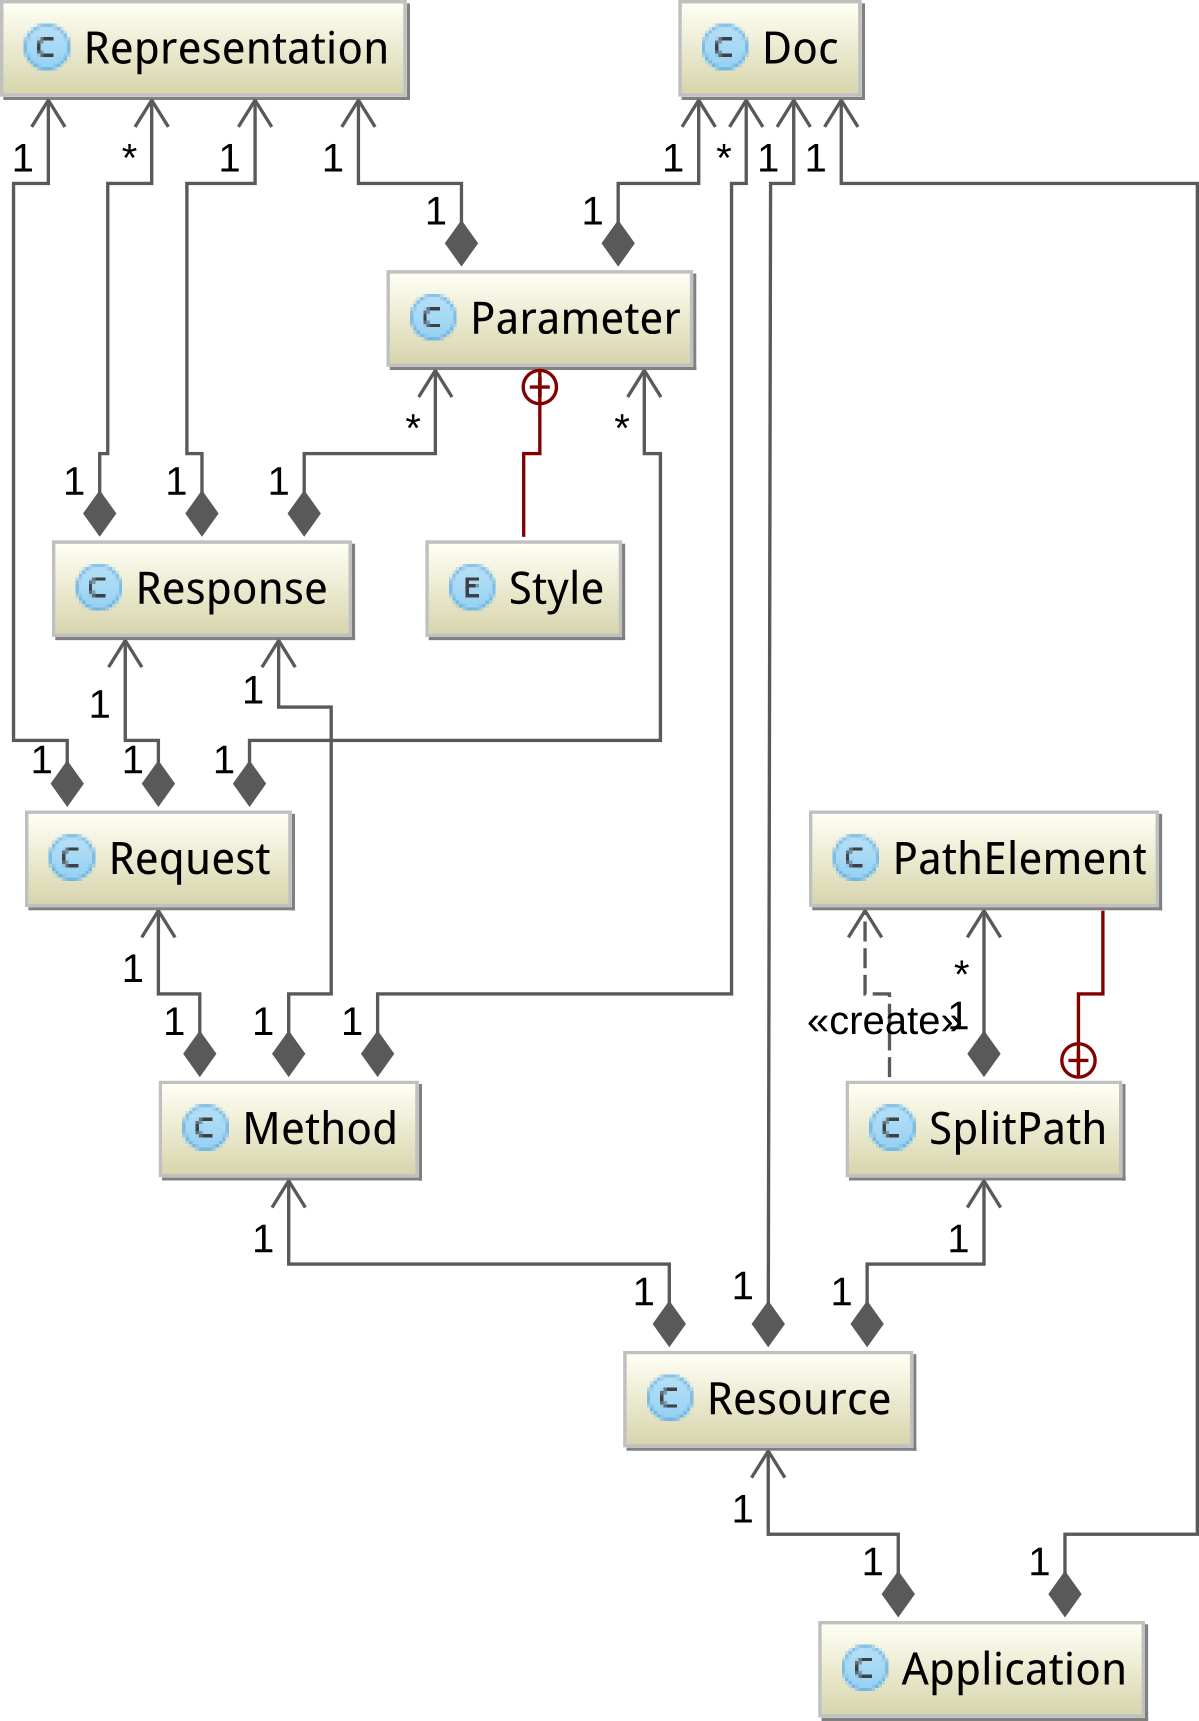
\includegraphics[width=0.5\textwidth]{resources/restmodel}
    \caption{\textsc{Uml} Klassendiagramm des \gls{REST}-Modells}
    \label{fig:restmodel}
\end{figure}

Wurzelelement des Modells (siehe \cref{fig:restmodel}) ist die Klasse \textbf{Application}, sie enthält \emph{Ressource}-Objekte und den Basisbezeichner der \gls{API} beispielsweise \texttt{\small http://api.spreadshirt.net/api/v1/}. 

Eine \textbf{Ressource}-Klasse enthält eine Menge von \emph{Method}-Objekten sowie einen Ressourcenbezeichner. Dieser ist relativ zum Basisbezeichner des Wurzelelements. Die Ressourcenbezeichner können \emph{Template-Parameter} enthalten. Diese werden bei einer Anfrage durch einen konkreten Wert ersetzt. Beispielweise enthält der Bezeichner für die Ressource eines bestimmten Users den Template-Parameter \texttt{\{userid\}}, vollständiger Ressourcenbezeichner \texttt{users/\{userid\}}. Ressourcenbezeichner werden durch die Klasse \textbf{SplitPath} repräsentiert. 

Jede \textbf{Method}-Klasse enthält ein \emph{Request} und ein \emph{Response} Objekt. Sie enthalten die nötigen Informationen für den Aufruf der Methode, beziehungsweise über den Aufbau der Antwortnachricht.

Eine \textbf{Request}-Klasse enthält eine Liste von Query-Parametern sowie ein \emph{Representation} und \emph{Response} Objekt.

\textbf{Parameter} enthält Angaben zum \emph{Style}, Typ, Vorgabewert und ob dessen Angabe \enquote{required}, also notwendig ist. Die Angabe des Typs ist eine Referenz auf einen Typ aus einer \gls{XML}-Schemabeschreibung. Der \emph{Style} gibt an wie der Parameter übermittelt wird, als Teil der Query \texttt{?mediaType=xml}, \emph{Key-Value Pair} des \gls{HTTP}-Header oder als \emph{Template-Parameter} des Ressourcenbezeichners. 

Die Klasse \textbf{Response} enthält eine Liste mit \emph{Representation}-Objekten und Parameter-Objekten. Die Objekte vom Typ Representation enthalten die Beschreibung der Daten, die bei einer erfolgreichen Anfrage an die Ressource zurückgesendet werden sowie die der Fehlermeldung, welche der Client anderenfalls erhält. Zwischen einer Fehlermeldung und einer erfolgreichen Anfrage kann anhand des Werts des \gls{HTTP}-Statuscodes unterschieden werden. Erfolgreiche Anfragen liefern in der Antwort meist einen Statuscode 200 \textbf{OK} oder 201 \textbf{Created} zurück, abhängig von der Anfragemethode. Die Response Parameter geben Einträge im \gls{HTTP}-Header an, welche für den Client nützliche Informationen enthalten. Legt der Client z.B. via \textsc{Post} auf der Ressource \texttt{sessions} eine neue \gls{API}-Session an, so enthält das Feld \texttt{Location} des \gls{HTTP}-Headers der Serverantwort eine \gls{URL} auf die Ressource der angelegten Session.

Die \textbf{Representation}-Klasse dient zur Beschreibung der Daten, welche entweder zur \gls{API} gesendet oder von dieser empfangen werden, sie besteht aus einer Angabe des \emph{media-type}, des \gls{HTTP}-Statuscodes und eine Referenz auf die Definition des Datentyps. Das \emph{Representation}-Objekt des Request einer \textsc{Put}- oder \textsc{Post}-Methode charakterisiert zum Beispiel den Aufbau der Daten, welche der Ressource übermittelt werden, üblicherweise im \gls{HTTP}-Body. Die Charakterisierung erfolgt dabei in Form einer Referenz auf einen Typ aus einer Schemabeschreibung sowie der Angabe des \emph{media-type}. Beispielsweise enthält das \emph{Representation}-Objekt der \textsc{Put}-Methode auf Ressource \texttt{users/\{userId\}/designs/\{designId\}} den media-type \texttt{application/xml} und eine Referenz auf den Typ \texttt{sns:design}. 

Referenzen auf Typdeklaration aus einer Schemabeschreibung werden nachfolgend im Modell durch die konkrete Deklaration des Typs aus der \gls{XML}-Schemabeschreibung ersetzt, siehe \cref{sec:application_model}. 

Ein Objekt der \textbf{Doc}-Klasse enthält einen Titel und eine Kurzbeschreibung des zugehörigen Elements.
Der Generator erzeugt daraus Quellcodekommentare für die Dokumentation der Bibliothek.